\documentclass{scrartcl}

% neccesarry for style
\usepackage[english]{babel}
\usepackage[utf8]{inputenc}
\usepackage[T1]{fontenc}
\usepackage{lmodern}

% tools for text
\usepackage{csquotes}
\usepackage{url}
\usepackage{hyperref}

% graphics
\usepackage{graphicx}
\usepackage{xcolor}
\usepackage{tikz}

% maths
\usepackage{amsmath,amssymb,amstext,amsthm}

% programming
\usepackage{listings}

\usepackage{wasysym} %lightning

\input{required/settings.tex}
\input{required/commands.tex}

\usepackage{pdflscape}

\renewcommand{\labelenumi}{\alph{enumi})}
\begin{document}
	\begin{center}
		\LARGE
		Information Integration -- Exercise 7 -- Gabriel Glaser
	\end{center}
	
	\section*{Task 3: Entity Resolution and Fusion (Sample exam question)}
	\begin{center}
			\fbox{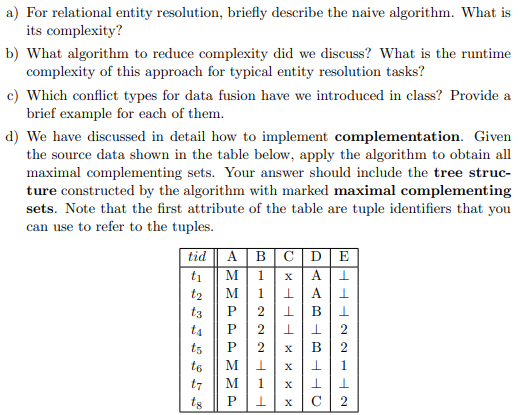
\includegraphics[width=0.9\textwidth]{figures/task3.PNG}}
	\end{center}
	\begin{enumerate}
		\item Pair-wise comparison of each entity (e.g., similarity measure + threshold) based on Cartesian product.
		This has a quadratic runtime complexity.
		
		\item Sorted-Neighbourhood reduces the complexity to $\mathcal{O}(n\log n)$.
		Calculate $n$ keys, sort ($n\log n$) and linear scan to find duplicate candidates in a constant window.
		
		\item\phantom{phantom}
		\begin{itemize}
			\item \textit{Exact duplicate}: No problem, can drop one of the entities (SQL UNION).
			For example,
			\begin{center}
				\begin{tabular}{|c|c|c|}
					\hline
					title & author & year\\
					\hline
					Harry Potter 1 & J.K. Rowling & 1996\\
					Harry Potter 1 & J.K. Rowling & 1996\\
					\hline
				\end{tabular}.
			\end{center}
			
			\item \textit{Subsumption}: One entity is the subset of the other entity.
			For example,
			\begin{center}
				\begin{tabular}{|c|c|c|}
					\hline
					title & author & year\\
					\hline
					Harry Potter 1 & J.K. Rowling & 1996\\
					Harry Potter 1 & J.K. Rowling &\\
					\hline
				\end{tabular}.
			\end{center}
			
			\item \textit{Complementation}: Either both entities contain the same value or only one entity has a value.
			For example,
			\begin{center}
				\begin{tabular}{|c|c|c|}
					\hline
					title & author & year\\
					\hline
					Harry Potter 1 & & 1996\\
					Harry Potter 1 & J.K. Rowling &\\
					\hline
				\end{tabular}.
			\end{center}
				
			\item D\textit{ata Conflict}: There is an attribute where two different values are provided.
			For example,
			\begin{center}
				\begin{tabular}{|c|c|c|}
					\hline
					title & author & year\\
					\hline
					Harry Potter 1 & J.K. Rowling & 1996\\
					Harry Potter and the Sorcerer's Stone & J.K. Rowling &\\
					\hline
				\end{tabular}.
			\end{center}
		\end{itemize}
		
		\item\phantom{phantom}
		\begin{itemize}
			\item $t_1, t_2, t_6, t_7$
			\item $t_3, t_4, t_5$
			\item $t_4, t_5$
			\item $t_4, t_8$
		\end{itemize}
	\end{enumerate}
	\begin{landscape}
		\pagestyle{empty}
		\begin{center}
			\hspace*{-5.5cm}
			\begin{tikz}[level 1/.style={sibling distance=3.7cm},
				level 2/.style={sibling distance=1.5cm},
				level 3/.style={sibling distance=1cm},
				level 4/.style={sibling distance=3cm}]
				\node[draw, circle] {\phantom{}}
				child{node[draw, circle]{$t_1$}
					child{node[draw, circle]{$t_2$}
						child{node[draw, circle]{$t_6$}
							child{node[draw, circle]{$t_7$}
							}
						}
						child{node[draw, circle, fill=gray]{$t_7$}
						}
					}
					child{node[draw, circle, fill=gray]{$t_6$}
						child{node[draw, circle, fill=gray]{$t_7$}
						}
					}
					child{node[draw, circle, fill=gray]{$t_7$}
					}
				}
				child{node[draw, circle, fill=gray]{$t_2$}
					child{node[draw, circle, fill=gray]{$t_6$}
						child{node[draw, circle, fill=gray]{$t_7$}
						}
					}
					child{node[draw, circle, fill=gray]{$t_7$}
					}
				}
				child{node[draw, circle]{$t_3$}
					child{node[draw, circle]{$t_4$}
						child{node[draw, circle]{$t_5$}
						}
					}
					child{node[draw, circle, fill=gray]{$t_5$}
					}
				}
				child{node[draw, circle, fill=gray]{$t_4$}
					child{node[draw, circle]{$t_5$}
					}
					child{node[draw, circle]{$t_8$}
					}
				}
				child{node[draw, circle, fill=gray]{$t_5$}
				}
				child{node[draw, circle, fill=gray]{$t_6$}
					child{node[draw, circle, fill=gray]{$t_7$}
					}
				}
				child{node[draw, circle, fill=gray]{$t_7$}
				}
				child{node[draw, circle, fill=gray]{$t_8$}
				};
			\end{tikz}
		\end{center}
	\end{landscape}
	
\end{document}
